\documentclass{article}
\usepackage{hyperref}

\usepackage[margin = 1in]{geometry}
\usepackage{listings}
\usepackage{mathtools}
\usepackage{apacite}
\usepackage{graphicx} \graphicspath{ {./Images/} }
\usepackage{blindtext}
\usepackage{titling}
\usepackage{setspace} \doublespacing
\usepackage{wrapfig} 
\setlength\parindent{24pt}
\renewcommand\maketitlehooka{\null\mbox{}\vfill}
\renewcommand\maketitlehookd{\vfill\null}



\title{Spiking Neural Networks}
\author{Arslan Salikhov \\
	\and 
	Erik Caceros \\
	\and
	Brandon Lam \\
	}
\date{\today}



\begin{document}

\begin{titlingpage}
\maketitle
\begin{abstract}
	Use of Deep Neural Network, commonly referred to as
	\emph{deep learning} spiked in recent years and has been used
	as a tool for impressive advancements in the field of 
	\emph{Artificial Intelligence (AI)}
	Spiking Neural Networks draw inspiration from the 
	Purpose of this project is to demonstrate the capabilities of a 
	Spiking Neural Network and compare it to a more conventional 
	Object Recognition Deep Neural Network
	\end{abstract}
\end{titlingpage}


\tableofcontents
\newpage




\section{Architecture of the Spiking Neural Network}

When it comes to building a neural network, one has to establish an
architecture or an arrangement of layers and how they connect with each other.
It is particularly important, when the network increases in complexity. Object
classification + localization being a demanding task for a network to solve,
we have adopted a published and well-tested architecture for the task --
ResNet. The particular architecture we have tried to imitate titled 
\textit{DECOLLE}, was first developed by \citeA{kaiser2018synaptic} and later
enhanced by \citeA{barchid2021deep}. \textit{DECOLLE} Neural Network adopts 
properties of classical ResNet model architecture as well as a pyramidal structure that
was proposed by \citeA{pyramid}. 

\subsection{ResNet}

\begin{wrapfigure}[21]{r}{0.42\textwidth}
\begin{center}
	\scalebox{0.35}{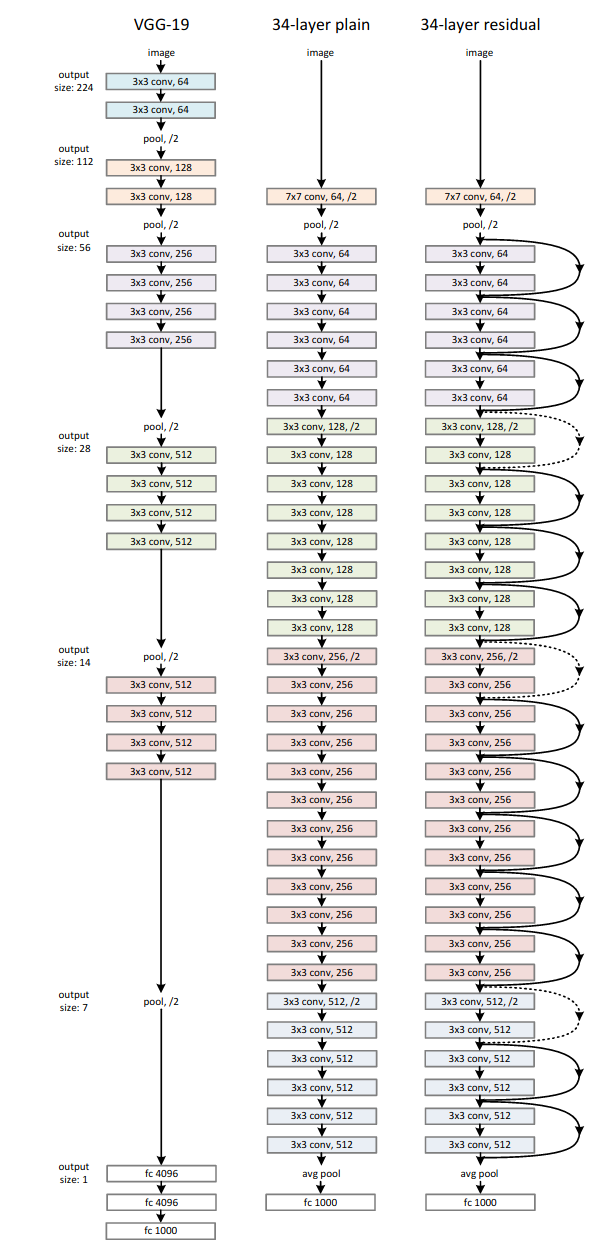
\includegraphics{resnet_comp.png}}
\end{center}
	\caption{Examples of 16-layer VGG, Plain 34-layer, and 34-layer ResNet Network 
	Architectures}
\end{wrapfigure}




To begin with the cornerstone of our architecture -- ResNet, it was named for its property,
of convolutional layers of the network that are residually connected with each other using
shortcut connections (\citeA{resnet}).
According to the authors of the original paper on ResNets,
addition of residual connections improves model's convergence, or ability for
model's loss to move towards a minimum with a decreasing trend. Meanwhile,
ResNets converge faster than their plain counterparts, the complexity of 
ResNets is much lower than complexity of well established Visual Geometry
Group (VGG) Networks given the same depth (3.6 billion FLOPs (Float Point 
Operations) vs. 19.6 billion FLOPs) (\citeA{resnet}). 

\subsection{Comparing Model Performance}
To compare networks' performance one has to understand how it is measured and what
constitutes an accurate model. For the task of object detection/localization accuracy
of the model at predicting class of the object in the image is not enough. Thus,
two additional performance metrics have been adapted : Mean Average Precision (mAP) and
Intersection of Union (IoU). Firstly, Mean Average Precision for the purposes of Object
Detection is well-defined in the paper by \citeA{evaluation}. According to the authors,
mAP is mean of Average Precision of the model for all the classes in the dataset.


\begin{equation}
	\textbf{mAP} = \frac{1}{N} * \sum_{i = 1}^{N} \textbf{AP}_i
\end{equation}

\begingroup
\fontsize{7pt}{9pt}\selectfont
\begin{enumerate}
	\item[]  \begin{center} \textit{AP = Average Precision,} \end{center}
	\item[] \begin{center}  \textit{N = number of classes.} \end{center}
\end{enumerate}
\endgroup

Moreover, ResNets perform better
than plain Deep Convolutional Networks in terms of accuracy. In order to compare 

\newpage
\bibliographystyle{apacite}
\bibliography{report}

\end{document}